\documentclass[a4paper,10pt]{article}
\usepackage[utf8x]{inputenc}

\usepackage{verse}
\usepackage[slovene]{babel}
\usepackage{graphicx}
\usepackage{hyperref}
\usepackage{amsmath}
\usepackage{amsfonts}
\usepackage{comment}
\usepackage{subfigure}

\newcommand{\slika}[2]{
\begin{figure}[h]
 \input{#1}
  \caption{#2}
  \label{fig:#1}
\end{figure}
}

\newcommand{\dd}{\,\mathrm{d}}

\title{Generatorji slu"cajnih "stevil}
\author{Miha \v Can\v cula}

\begin{document}
 \maketitle

\begin{abstract}
 The generation of random numbers is too important to be left to chance.
     -- Robert R. Coveyou, \textit{Oak Ridge National Laboratory}
\.\\
\begin{figure}[h!]
\centering
  \subfigure{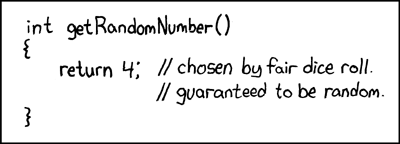
\includegraphics[width=250pt]{random-xkcd}}\\
  \subfigure{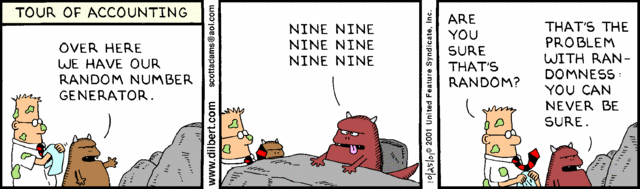
\includegraphics[width=300pt]{random-dilbert}}
\end{figure}
\end{abstract}

\section{Enakomerne porazdelitve}

Najenostavnej"sa je bila primerjava med generatorji, ki vrnejo naklju"cna "stevila, ki so enakomerno razporejena po nekem intervalu. Tak"snih generatorjev je tudi najve"c, zato sem jih lahko primerjal. Za vsakega sem izra"cunal porazdelitev verjetnosti z razdelitvijo v 100 predal"ckov, nato pa na ti porazdelitvi izvajal statisti"cne teste. Uporabil sem naslednje generatorje:

\begin{enumerate}
 \item Funkcija \texttt{rand()} iz standardne knji"znice jezika \texttt{C}
 \item Linuxova datoteka \texttt{/dev/urandom}
 \item Kalkulatorski generator, opisan v navodilih
 \item ``Mersennov vrtinec'', implementiran v \texttt{GSL} 
\end{enumerate}

Poleg teh generatorjev sem za primerjavo vklju"cil "se dva izvora naklju"cnih "stevil, ki "stevil ne generirata s "stevilskim algoritmom, ampak jih izra"cunata te"zko predvidljivih dogodkov. V nasprotju z generatorji na ta na"cin ne moremo dobiti poljubnega "stevila naklju"cnih "stevil, zato sem velikost vzorca omejih na 4096 "stevil, kjer ima vsako "stevilo 32 bitov.

\begin{enumerate}
 \item Linuxova datoteka \texttt{/dev/random}, ki naklju"cnost dobi iz dogodkov v ra"cunalniku, na primer s premikanjem mi"ske
 \item Spletna stran \texttt{random.org}, ki naklju"cnost dobi iz meritev atmosferskega "suma
\end{enumerate}

\begin{table}[h]
 \centering
  \begin{tabular}{|c|c|c|c|c|c|c|c|c|c|}
  \hline
  Test & \multicolumn{3}{|c|}{Enodimenzionalni $\chi^2$} & \multicolumn{3}{|c|}{Dvodimenzionalni $\chi^2$} & \multicolumn{3}{|c|}{Kolmogorov-Smirnov} \\
  \hline
  Velikost vzorca & $2^{12}$ & $2^{18}$ & $2^{24}$ & $2^{12}$ & $2^{18}$ & $2^{24}$ & $2^{12}$ & $2^{18}$ & $2^{24}$ \\
  \hline
  \texttt{rand()} & \\
  \texttt{/dev/urandom} & \\
  Kalkulatorski & \\
  Mersenne & \\
\hline
  \texttt{/dev/random} & \\
  \texttt{random.org} & \\
\hline
   
  \end{tabular}
\caption{Statisti"cni testi enakomernosti naklju"cnih "stevil}
\end{table}

\section{Smeri v prostoru}

Za generacijo naklju"cnih meri v prostoru najprej potrebujemo generator enakomernih naklju"cnih "stevil. V ta namen sem uporabil kar najbolj"si generator iz prve naloge, to je bil Mersennov vrtinec. Knji"znica \texttt{GSL} ima vgrajeno rutino, ki s pomo"cjo enakomernega generatorja vrne naklju"cen enotski vektor v treh dimenzijah. Kljub temu pa sem za primerjavo "se sam napisal tak"sen generator. Za primer brez sevanja je algoritem enostaven, saj vemo da mora biti porazdelitev verjetnosti enakomerna po spremenljivkah $\varphi$ in $\cos\vartheta$. "Ce sta $r_1$ in $r_2$ dve naklju"cni "stevili z intervala $[0,1)$, lahko prostorski kot zapi"semo kot

\begin{align}
 \varphi &= 2\pi r_1 \\
 \vartheta &= \arccos (2r_2-1)
\end{align}

Pri dipolnem sevanju je porazdelitev verjetnosti po kotu $\vartheta$ bolj zapletena. 

\begin{align}
 \frac{\partial p}{\partial \vartheta} & \propto \sin^3\vartheta \\
  \dd p &= A \sin^3 \vartheta \dd \vartheta = A(1-\cos^2\vartheta) \dd (\cos\vartheta) \\
&= A \dd\left( \cos\vartheta - \frac{\cos\vartheta^3}{3} \right)
\end{align}

"Ce upostevamo, da je $r_2$ enakomerno razporejen, dobimo ena"cbo za $\vartheta$. 

\begin{align}
\frac{\cos^3\vartheta}{3} - \cos\vartheta + A(r_2 - x_0) = 0
\end{align}


Da izrazimo $\cos\vartheta$ s pomo"cjo $r_2$ bomo morali re"sitiv polinom tretje stopnje. Iz pogoja $\int\!\!\dd p=1$ in upo"stevanja omejitve $\cos\vartheta \in [-1,1]$ dolo"cimo konstanti $A$ in $x_0$. 

\section{Gaussova porazdelitev}

Tu je postopek podoben kot pri generiranju naklju"cnih smeri. Uporabimo generator enakomerno porazdeljenih "stevil, ki jih transformiramo na tak na"cin, da bo porazdelitev transformirank Gaussova. V ta namen se najve"c uporabljata Box-Mullerjeva transformacija in metoda ``zigurat''. 

\end{document}
